\chapter{LHC Olympics 2020 Dataset}\label{chap:Dataset}

\section{ATLAS coordinate system}\label{sec:CoordinateSystem}
The dataset we use to develop this thesis is composed by positions and momenta of simulated particles originating after a collision. For this reason, prior to discussing its structure, it would be appropriate analysing the coordinate system active in a particle detector, such as the ATLAS experiment \cite{PhDFrattari}\cite{ATLASexp}. In figure \ref{fig:CoordinateSystem} an overview of the system is presented.

\begin{figure}[h!]
    \centering
    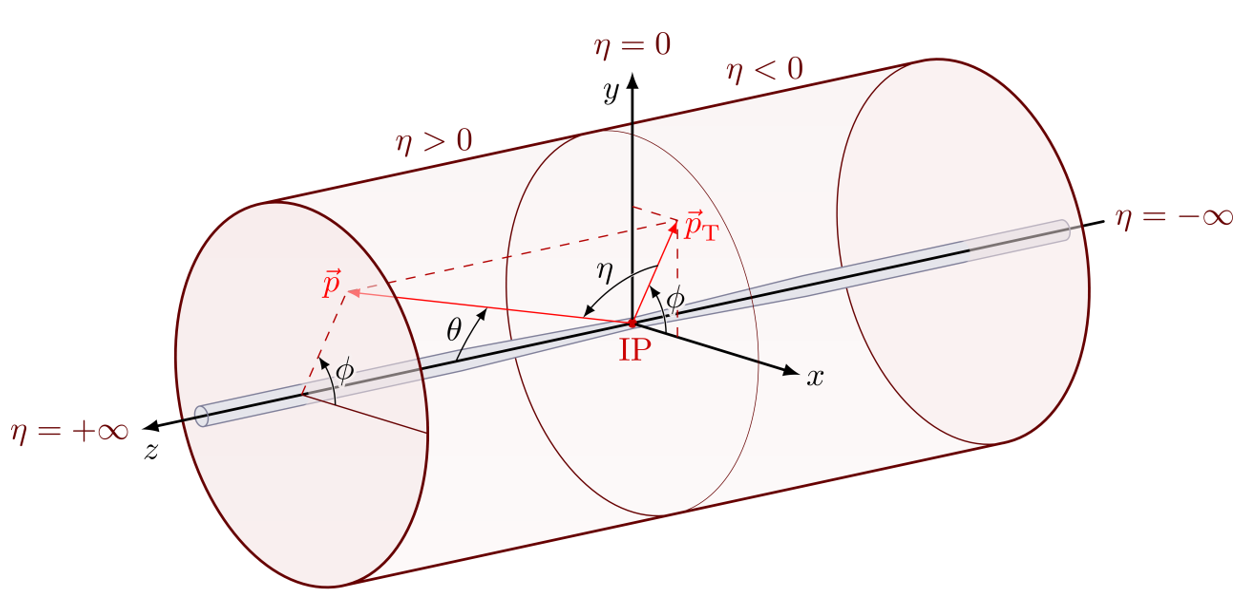
\includegraphics[width=4 in]{OLD/Images/Cap4/CoordinateSystem.png}
    \caption{Schematic of ATLAS coordinate system}
    \label{fig:CoordinateSystem}
\end{figure}

\noindent Cartesian axes (\textit{x,y,z}) are constructed as follows. The origin is set in the interaction point (IP). From it, the z-axis departs parallel to the beam tunnel with positive z-values in anticlockwise direction. As direct consequence, the x-y plane is perpendicular to it, with positive x-values towards the center of the LHC and positive y-values upward. On this Cartesian system, a cylindrical coordinate system ($r , \eta ,  \phi $) is defined to describe geometric position and components of particle momenta. $\phi$ is the azimuth angle, measured around the z-axis, with values [$-\pi , \pi $]. $\eta$ is named pseudo-rapidity and it is linked to the polar angle $\theta$ by the equation below:

\begin{equation}\label{eq:eta}
    \eta = - ln \Big( tan \frac{\theta}{2}\Big)
\end{equation}

\noindent The pseudo-rapidity and the azimuth angle, known as geographical coordinates \cite{ATLASexp}, are used to define a geometrical distance, applied when computing the separation between two physics objects:

\begin{equation} \label{eq:distance}
    \Delta R=\sqrt{\Delta \eta ^2 + \Delta \phi ^2}
\end{equation}

\noindent The third coordinate, $r$, is the radius from the center of the system. Actually, in this thesis, we use another information: the transverse momentum $p_T$. It is a 2D vector defined as the projection of the momentum in the transverse plane of the interaction. This parameter is related to the radius and it is important because it brings information about energy. In figure \ref{fig:pT} it is possible to observe how $p_T$ is calculated.


\begin{figure}[h!]
    \centering
    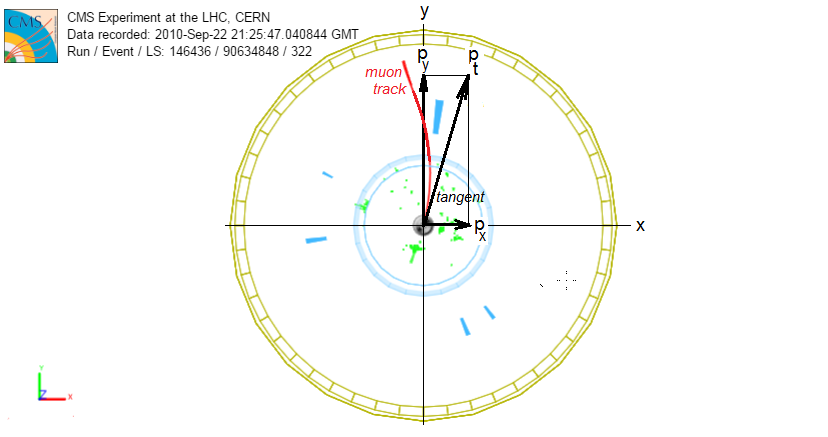
\includegraphics[width=3 in]{OLD/Images/Cap4/TransverseMomentum.png}
    \caption{Schematic of $p_T$ computing in the CMS experiment, analogous  to ATLAS}
    \label{fig:pT}
\end{figure}

%%%%%%%%%%%%%%%%%%%%%%%%%%%%%%%
\section{LHC Olympics Dataset}\label{sec:LHCDataset}

In this thesis we deal with the R\&D dataset created for the LHC Olympics 2020 \cite{LHCOlympics}, a challenge promoted by CERN collaboration to contribute to New Physics searches. It is made up of 1 million background events and 100 000 signal events, the anomalies we are looking for. The background is associated to SM phenomena, especially quantum chromodynamics (QCD) dijet events. The signal is about the resonance of $Z'$ particle: $Z' \rightarrow XY$, with $X \rightarrow q\Bar{q}$ and $Y\rightarrow q\bar{q}$. The masses of the particles are: $m_{Z'}$= 3.5 TeV, $m_X$= 500 GeV, $m_Y$= 100 GeV.  The topology of the interaction is presented in figure \ref{fig:Feynman}

\begin{figure}[h!]
    \centering
    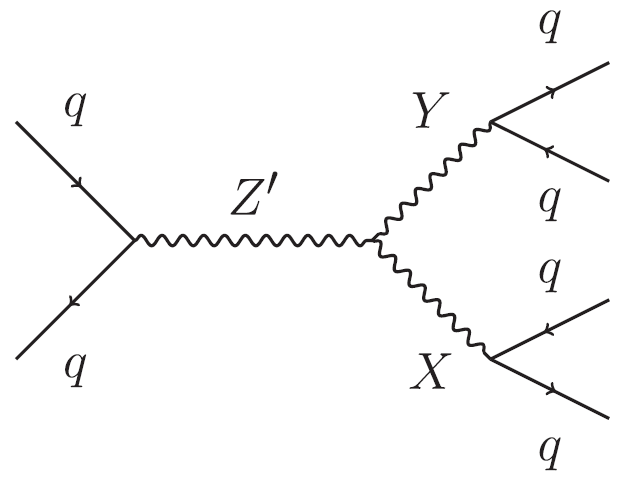
\includegraphics[width= 2in]{OLD/Images/Cap4/FeymanSignal.png}
    \caption{Topology of the signal interaction. Figure from Ref. \cite{LHCOlympics}}
    \label{fig:Feynman}
\end{figure}

\noindent A resonance is used in the signal dataset because the dijet final state offers a complex topology for hiding new physics.\\
The dataset is produced in Monte Carlo (MC) simulations using Pythia 8.219 and Delphes 3.4.1 with default settings, simulating an ideal particle detector. Events are selected using an anti-$k_t$ jet trigger with R=1 and a $p_T$ threshold of 1.2 TeV.\\
For each event we have information about up to 700 particles and for each of them, we have three features, $p_T$, $\eta$ and $\phi$. Zero padding is applied, meaning that if an event has less then 700 physical data, zeros are added in order to get a perfect rectangle. Together with spatial information, a truth value is appended to every event in order to know whether it is a background (value=0) or a signal event (value=1). In conclusion the dataset has shape: (1.1 M, 2101).\\

%%%%%%
\subsection*{Jet clustering}\label{sec:JetClustering}
Quarks in the final state of our events (both background and signal) hadronize in the calorimeters. This phenomenon induces sprays of particles in the detector, defined jets. Prior to applying AD, data needs to be pre-processed in order to reconstruct jets. The reconstruction is performed applying the anti-$k_t$ algorithm \cite{antikT}. This method relies on the distance $d_{ij}$ between two constituents ($i, j$) and the distance $d_{iB}$ between a jet $i$ and the beam B:

\begin{equation} \label{eq:distanceantikT}
\begin{split}
    d_{ij}=min\big(p^{2k}_{Ti},p^{2k}_{Tj}\big)\frac{\Delta^2_{ij}}{R^2}\\
    \Delta^2_{ij} = {(y_i - y_j )}^2 + (\phi_i - \phi_j )^2\\
    d_{iB}=k^{2p}_{ti} \ \rm \rm \ \rm \ \rm \ \rm \ \rm \ \rm \rm \ \rm \ \rm \ \rm \ \rm 
\end{split}
\end{equation}

\noindent where, working with the constituent i, $p_{Ti}$ is its transverse momentum , $y_i$ is its rapidity and $\phi_i$ its azimuth; R is the radius parameter of the algorithm and $k$ is an additional parameter, equal to -1 in case of anti-$k_t$ algorithm, about the power of energy.

\begin{figure}[h!]
    \centering
    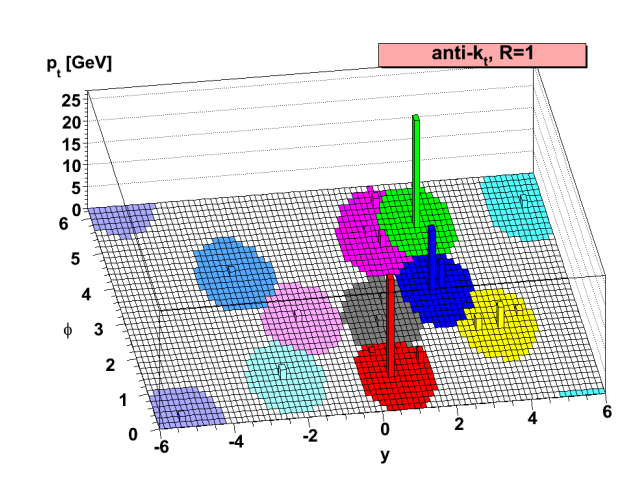
\includegraphics[width=3 in]{OLD/Images/Cap4/antikT.png}
    \caption{Example of anti-$k_t$ application. Figure from Ref. \cite{antikT}}
    \label{fig:antikt}
\end{figure}

\noindent We apply the anti-$k_t$ algorithm in this thesis using the Fastjet implementation and the radius parameter is set to R=1.\\
After the reconstruction, for each "physical" event we select the two most intense jets, defined as leading jet and sub-leading jet, if present. This means that the dimension of the whole dataset is multiplied by 2, becoming 2.2 M events. For each event we select up to 50 constituents and for each of them we still have the three features ($p_{Tfrac}  , \eta , \phi$), where $p_{Tfrac}=\frac{p_{Tconst}}{p_{tjet}}$ . Zero padding is applied and the truth value is preserved. The new shape of the dataset is (2.2 M, 50, 3),  with 2 M background events and 200k signal events.\\
In figure \ref{fig:DataDistNOTRANSF} it is possible to look at the distributions of the three features constituting the reconstructed dataset, for both background and signal events. In this plot events with $p_{Tfrac}$, and then $\eta$ and $\phi$, equal to zero are excluded, because they are not physical but just padding data.

\begin{figure}[h!]
    \centering
    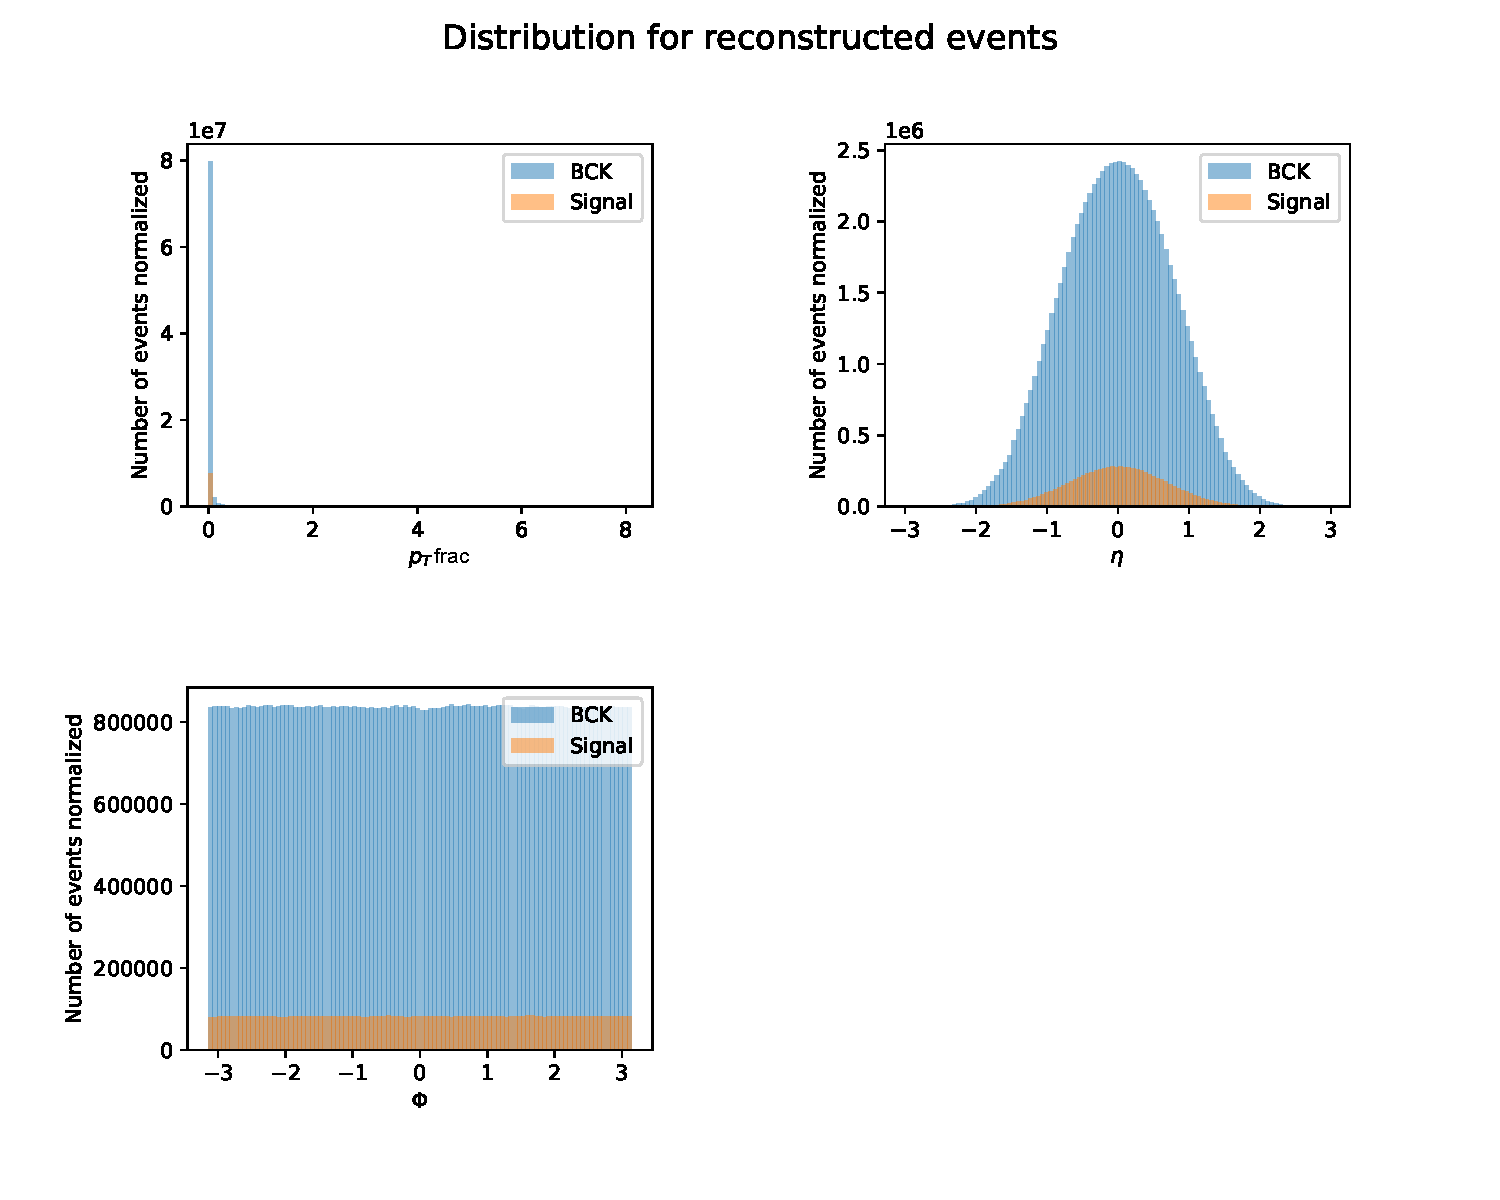
\includegraphics[width=5.1 in]{OLD/Images/DataDistribution/DataDistributionNOTRANF.pdf}
    \caption{Distribution for reconstructed events}
    \label{fig:DataDistNOTRANSF}
\end{figure}

\noindent To properly train our model and avoid misclassification error, data is scaled before moving to the next phase of the project. Data scaling is executed applying a standardization, implemented through the Standard Scaler function \cite{StandardScaler}, leading to a dataset with mean equal to 0 and standard deviation equal to 1. The task is completed passing each data x to the following equation:

\begin{equation}\label{eq:StandardScaler}
    z=\frac{x-\mu}{\sigma}
\end{equation}

\noindent where $\mu$ is the mean of the original dataset, $\sigma$ its standard deviation and $z$ is the scaled data. The new data distribution is presented in figure \ref{fig:DataDistNOTRANSFnorm}, where also jets with $p_T$=0 are plotted.\\

\begin{figure}[h!]
    \centering
    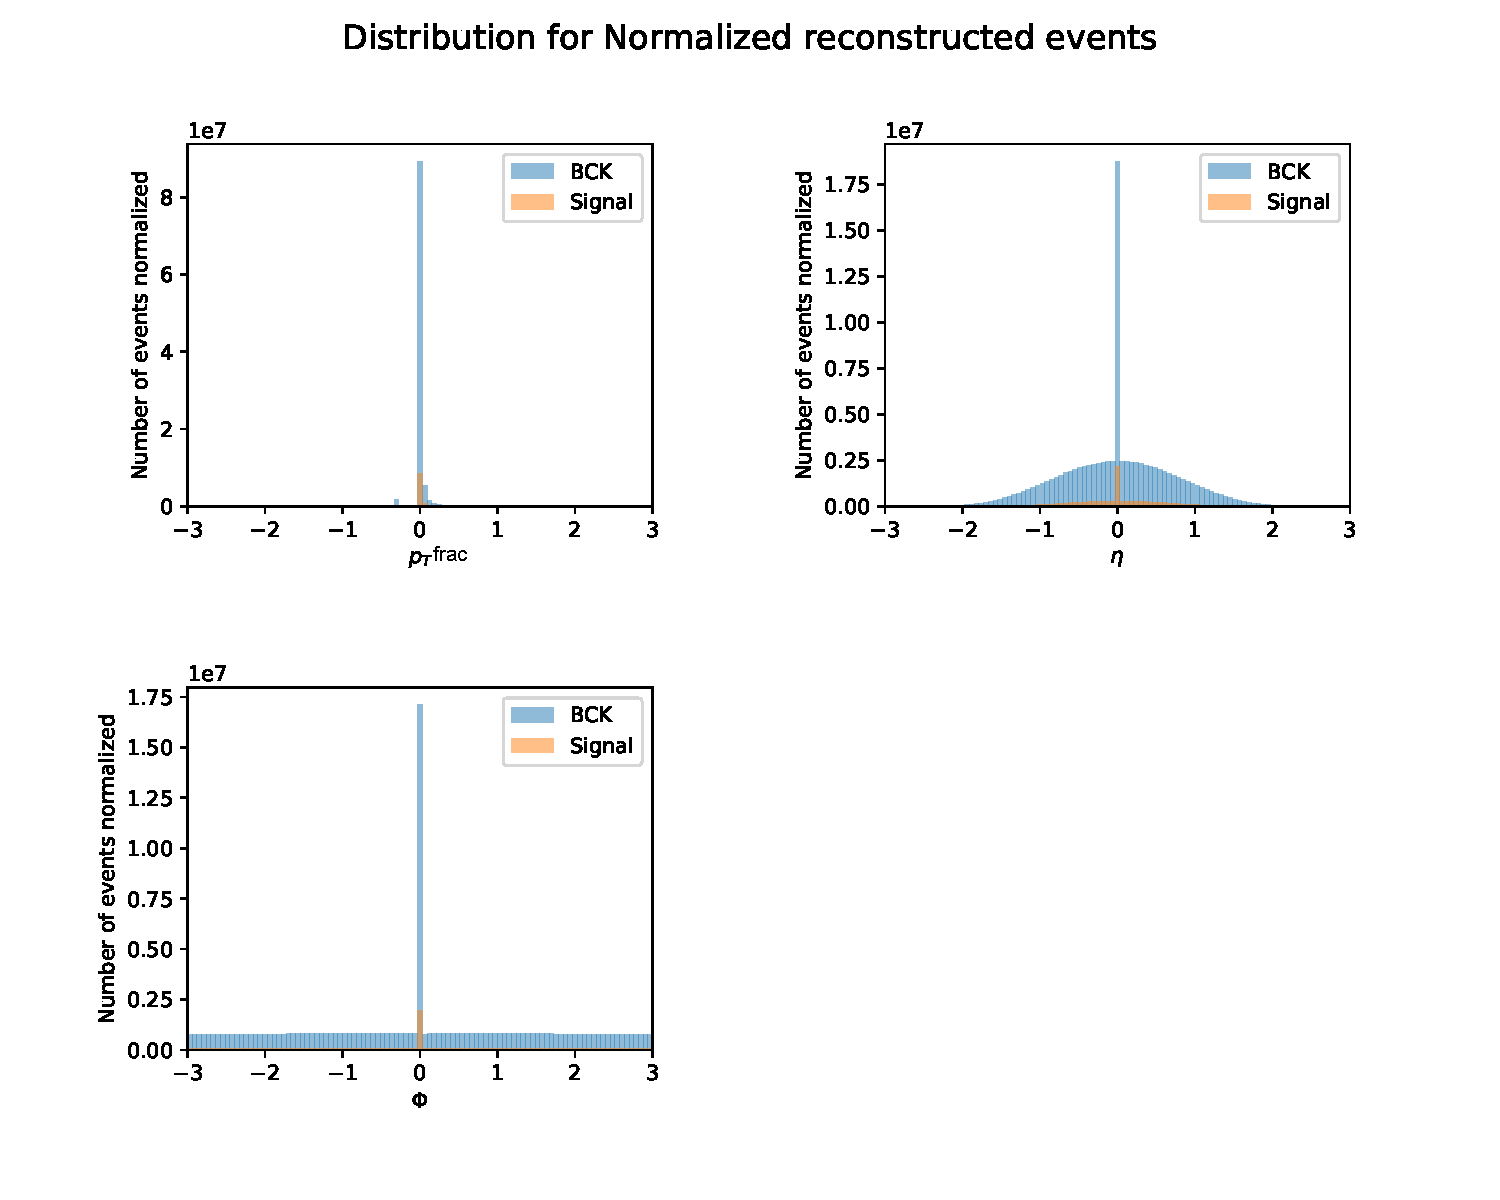
\includegraphics[width=5 in]{OLD/Images/DataDistribution/DataDistributionNOTRANFnorm.pdf}
    \caption{Distribution for reconstructed and normalized events}
    \label{fig:DataDistNOTRANSFnorm}
\end{figure}

%%%%%%%
\subsection*{Jet transformation}\label{sec:Transformation}
%%Among data there are jets with rotational symmetries, meaning there are jets physically identical but rotated. 
At this point of the thesis it is essential to admit that we want to focus on the micro-structures of a jet, based on the assumption that New Physics could be found there. Therefore the absolute position of the jet in the ($\eta, \phi$) plane is irrelevant, resulting in rotational symmetries among data. To study the impact of these symmetries either we let our model learn them (using the dataset described above) or we prepare new dataset removing them. One dataset is created applying a rotation; we will refer to it as the "rotated" dataset. The other is created to determine the correlation of mass with training results; we will call it the "transformed" dataset.\\
The rotation, is implemented using two Lorentz boosts. Given the coordinates of the jets $\eta_{jet}$ and $\phi_{jet}$, two Lorentz boost are applied consecutively in order to obtain $\eta'_{jet}=0$ and $\phi'_{jet}=0$. They are applied to all constituents of the jet. In figure \ref{fig:DataDistROT} and \ref{fig:DataDistROTnorm} new distribution plots are presented.

\begin{figure}[h!]
    \centering
    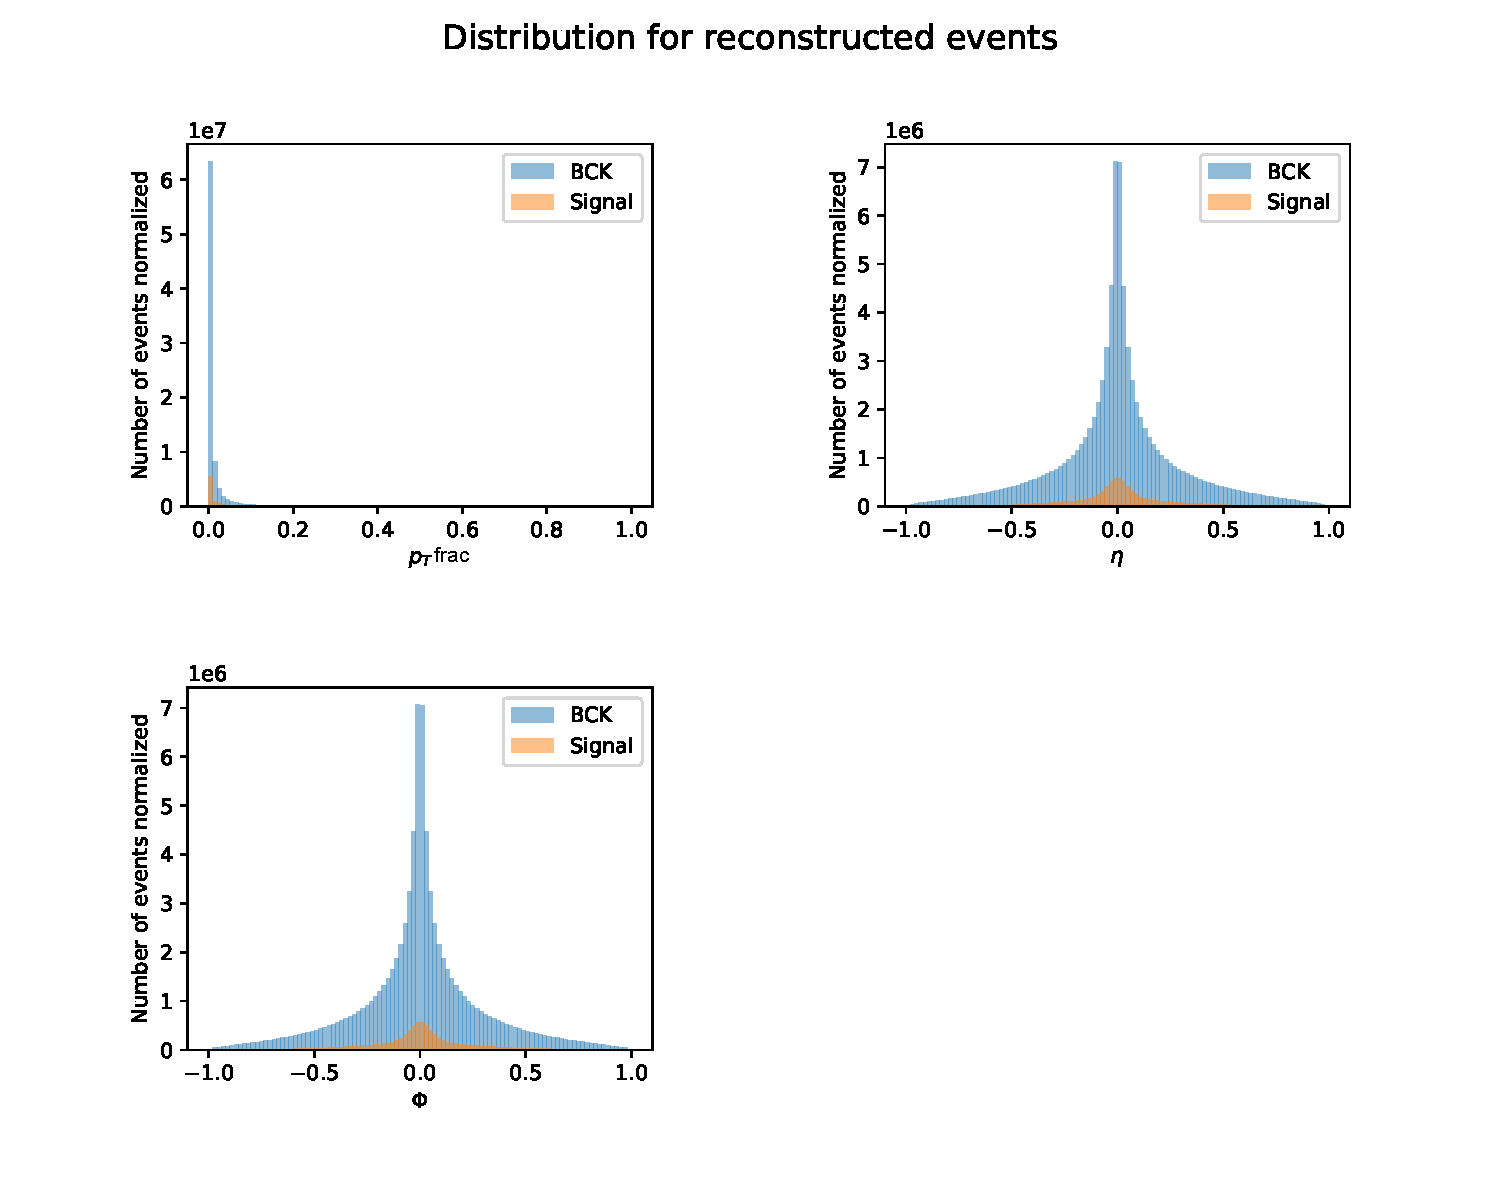
\includegraphics[width=4.7 in]{OLD/Images/DataDistribution/DataDistributionROT.pdf}
    \caption{Distribution for reconstructed and rotated events}
    \label{fig:DataDistROT}
\end{figure}

\begin{figure}[h!]
    \centering
    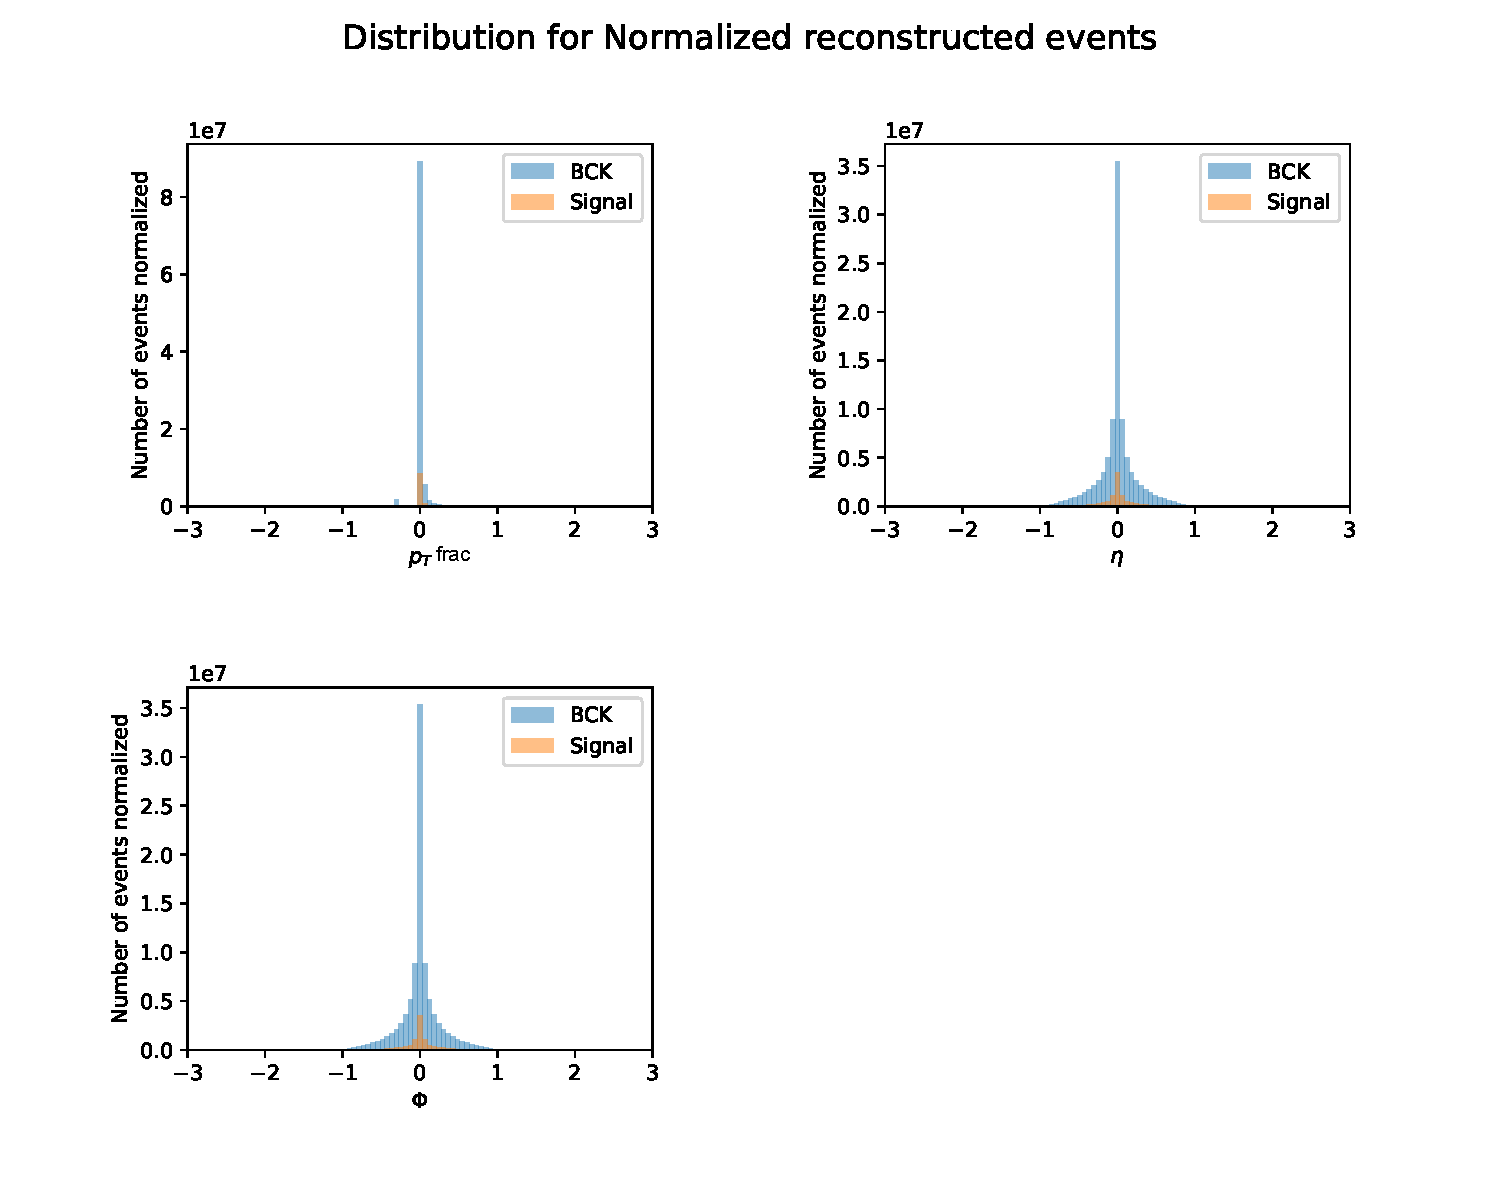
\includegraphics[width=4.7 in]{OLD/Images/DataDistribution/DistributionNORMROT.pdf}
    \caption{Distribution for reconstructed, rotated and normalized events}
    \label{fig:DataDistROTnorm}
\end{figure}

\noindent The transformation consists of few steps \cite{recoALGO}.\\
Prior to describing this method, a proper notation needs to be introduced. $P_J^{\mu}$ ($\Vec{P}_J$) is the four-momentum (three-momentum) of the jet, $p_i^{\mu}$ ($\Vec{p}_i$) is the same entity but related to the $i^{th}$ constituent. These vectors are used to describe the energy of the jet:
\begin{equation}\label{eq:4momenti}
    P_J^{\mu}=\sum^{N_J}_{i=1}p_i^{\mu}\ \rm ,\ \rm \ \rm   m_j^2=|P_J^{\mu}|^2= \big(P^0_J\big)^2 - \big(\overrightarrow{P}_J\big)^2 \ \rm ,\ \rm \ \rm E_J=P^0_J
\end{equation}

\noindent where $N_J$ is the number of constituents, $m_J$ is the jet mass and $E_J$ the jet energy.\\
First of all, we rescale the jet constituent four-momenta in order to set the jet mass to a value $m_0$=250 MeV:

\begin{equation}\label{eq:rescale}
   p_i^{ \mu} \rightarrow p_i^{' \mu}= \frac{m_0}{m_J}p_i^{\mu}\ \rm, \ \rm \ \rm P_J^{ \mu} \rightarrow P^{' \mu}_J= \frac{m_0}{m_J}P_J^{\mu}\ \rm,\ \rm \ \rm E_J \rightarrow E^{'}_J= \frac{m_0}{m_J}E_J
\end{equation}

\noindent Secondly, a Lorentz boost ($\Lambda^{\mu}_{\nu}$) is performed to set the energy of all jets to a value $E_0$= 1 GeV in the new frame of reference:

\begin{equation}\label{eq:LorentzBoost}
   p_i^{' \mu} \rightarrow \textbf{p}_i^{\mu}= \Lambda^{\mu}_{\nu}p_i^{' \nu}\ \rm, \ \rm \ \rm P_J^{' \mu} \rightarrow \textbf{P}^{\mu}_J= \Lambda^{\mu}_{\nu}P_J^{' \nu}\ \rm,\ \rm \ \rm \textbf{E}_J=\textbf{P}^0_J=E_0
\end{equation}

\noindent where letters in bold are associated to boosted jets. In conclusion, the rotation is applied. The distribution of the transformed dataset is visible in figure \ref{fig:DataDistTRANSF} and \ref{fig:DataDistTRANSFnorm}.

\begin{figure}[h!]
    \centering
    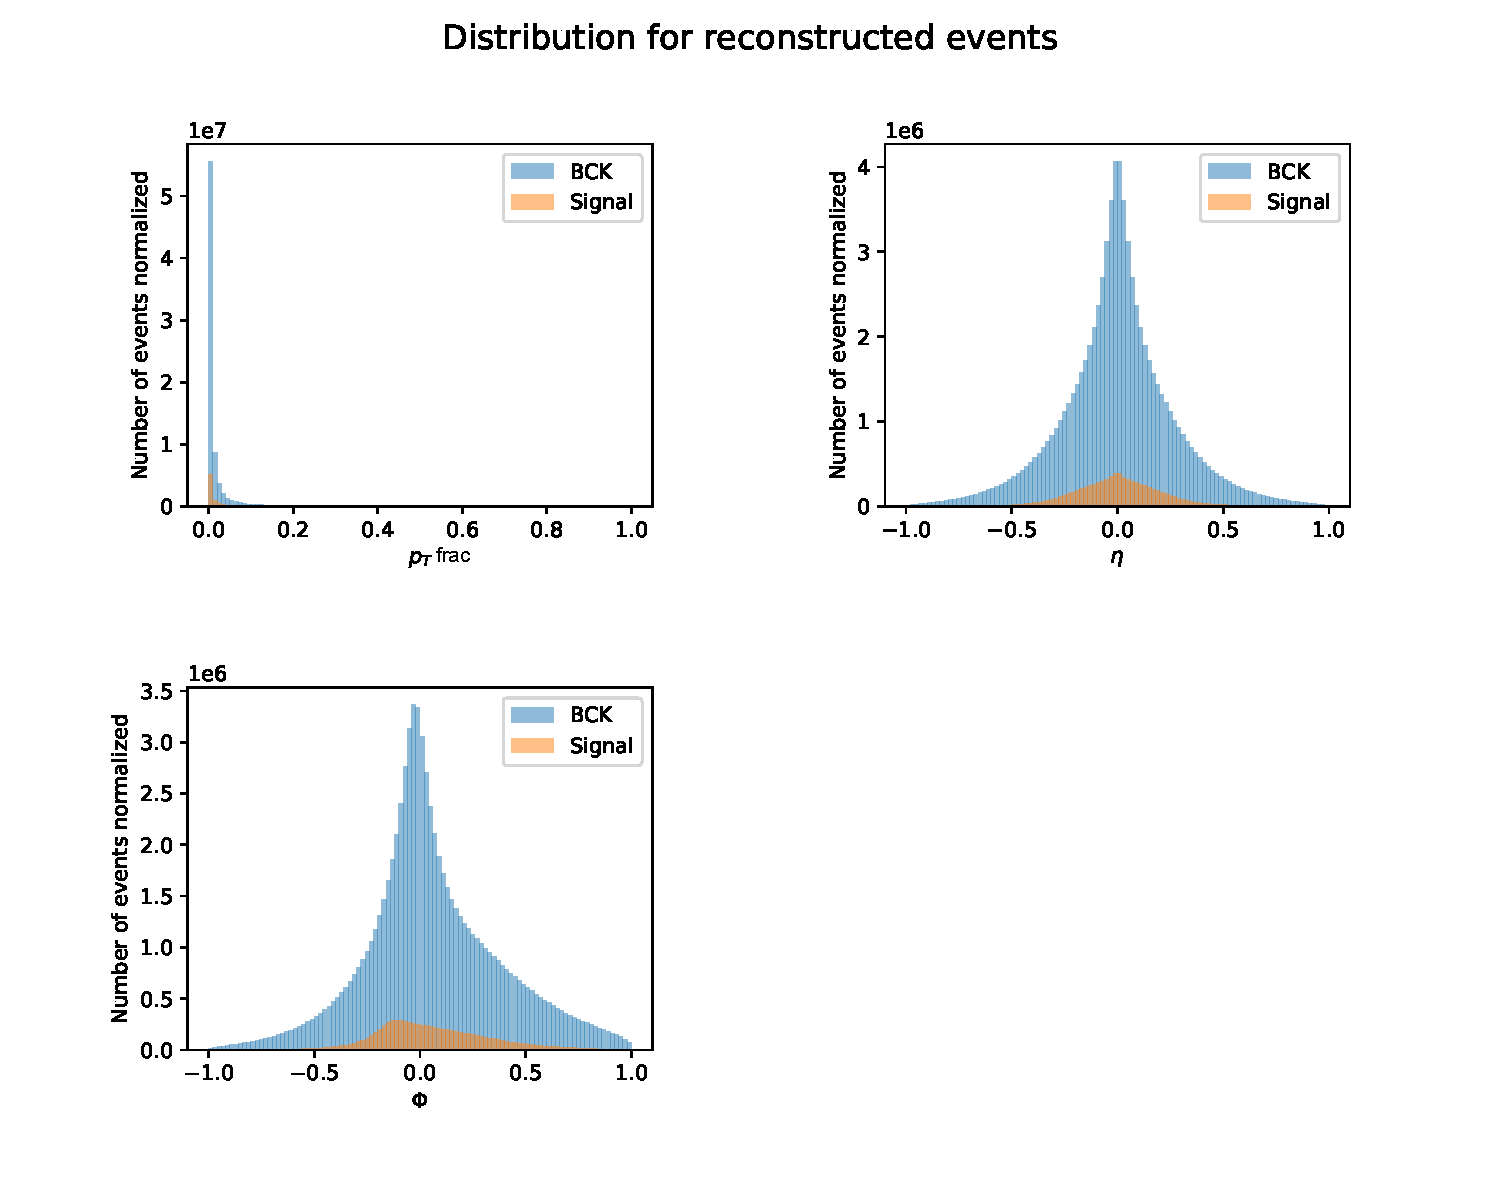
\includegraphics[width=5.2 in]{OLD/Images/DataDistribution/DataDistributionTRANSF.pdf}
    \caption{Distribution for reconstructed and transformed events}
    \label{fig:DataDistTRANSF}
\end{figure}

\begin{figure}[h!]
    \centering
    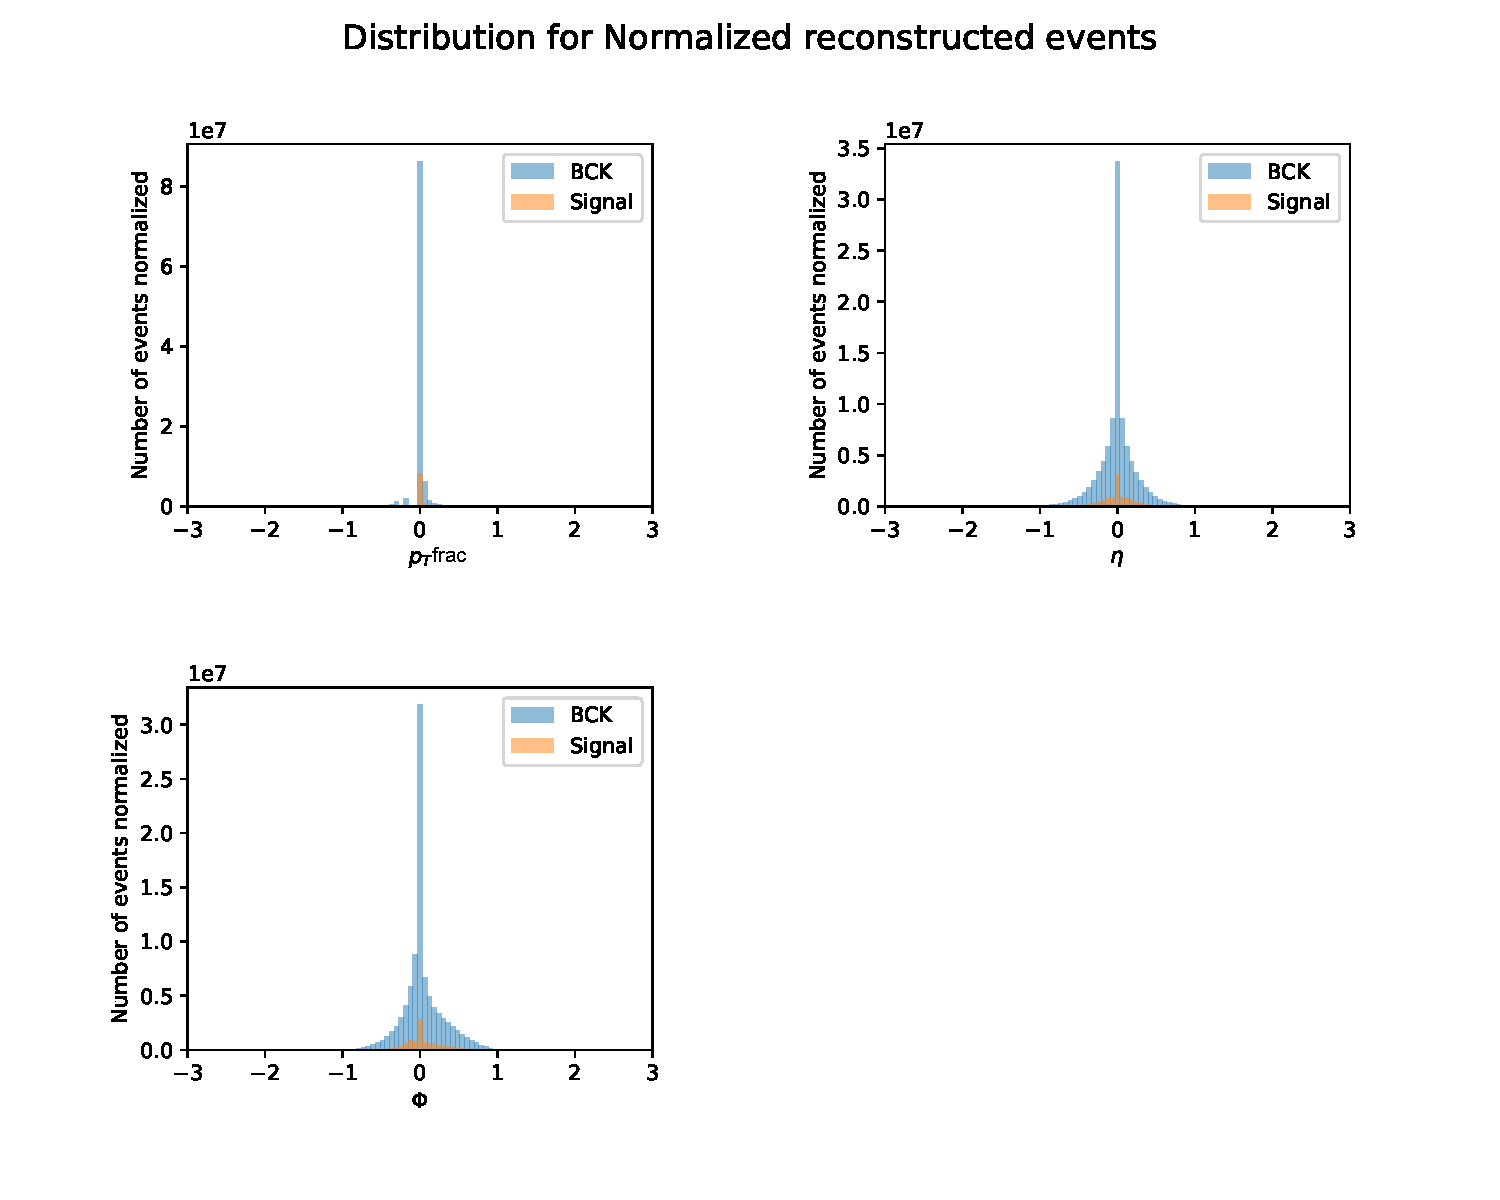
\includegraphics[width=5.2 in]{OLD/Images/DataDistribution/DistributionNORMTRANSF.pdf}
    \caption{Distribution for reconstructed, transformed and normalized events}
    \label{fig:DataDistTRANSFnorm}
\end{figure}


\noindent At this point, we expect our model to perform better and to be able to distinguish between the two kind of events. Our hope relies on the fact that we removed rotational symmetries and for kinematic reasons \cite{Bini}, all jets will be pushed forward and they will have a smaller spatial aperture, given the fact that the new energy of jets $E_0$ is lower than original energy. This feature will help our model during training, allowing it to focus on details and small differences. 

